\section{Bahrain Grand prix}

\subsection{Circuit Analysis}

\textbf{Circuit Name:} Bahrain International Circuit (Sakhir, Bahrain) \\
\textbf{Length:} 5.412 km - \textbf{Laps:} 57 - \textbf{Total Distance:} 308.238 km

\begin{figure}[H]
    \centering
    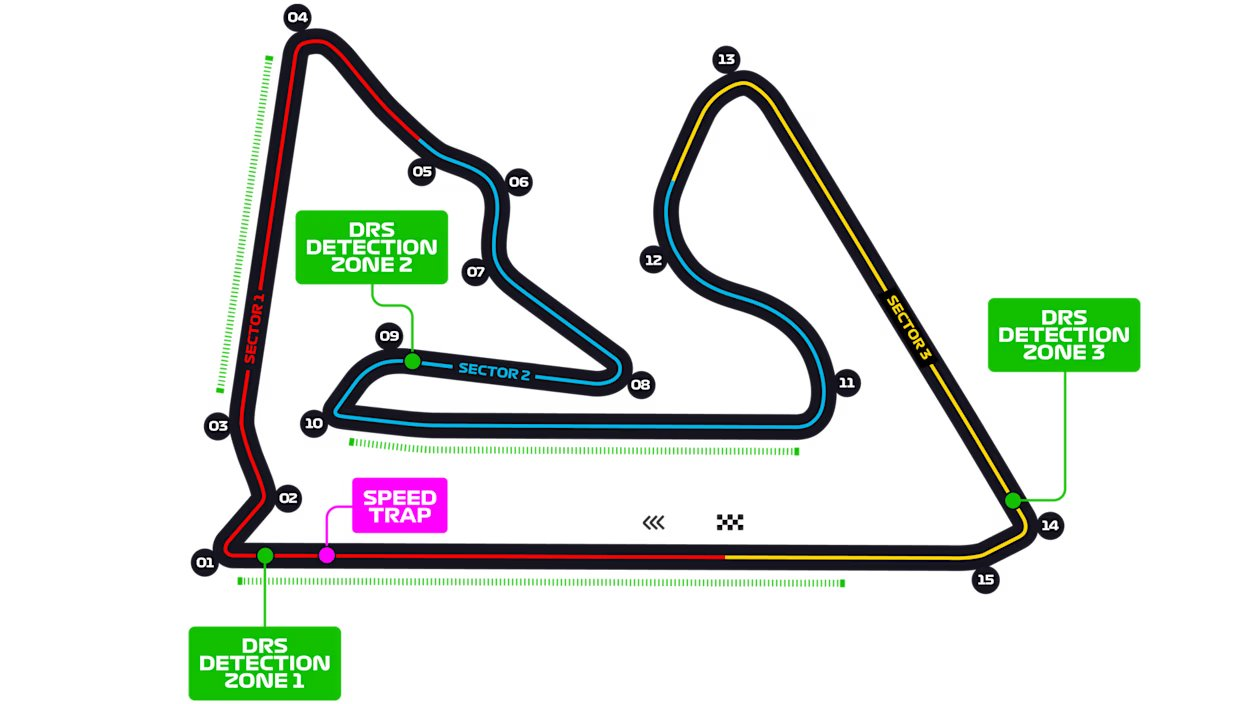
\includegraphics[width=0.75\linewidth]{images/1.Bahrain_Circuit.jpg}
\end{figure}

\begin{itemize}
    \item \textbf{Lap Record} : 1:27.264 (2020, Lewis Hamilton - Mercedes).
    
    \item \textbf{Number of Corners \& Key Features} : 15 turns (9 right, 6 left) - Track offers long straights, heavy braking zones (Turns 1, 4 \& 14), and technical sections like Turn 10 (off-camber, downhill)—key for grip and balance.
    
    \item \textbf{Braking Zones \& Traction} : Drivers brake from over 300 km/h to ~60 km/h in crucial zones, requiring extreme precision.\\
    Turn 10 particularly punishes front-left tyre instability.
    
    \item \textbf{DRS \& Overtaking} : Three DRS zones: along main straight, near Turn 4, and around Turn 10 areas. \\
    Combined with heavy braking zones, the track enables solid overtaking opportunities.
    
    \item \textbf{Tyre Degradation \& Strategy} : Teams chose mostly hard and soft compounds, medium rarely used. \\
    Two-stop strategies dominated: Soft–Hard–Soft or Soft–Hard–Hard favoured.
    
    \item \textbf{Weather \& Environment} : Night race with significant temperature swings and desert wind affects grip, braking stability, and tyre management.
\end{itemize}

\textbf{Strategic Summary :}
Bahrain demands cars with strong braking stability, rear traction, and efficient thermal regime. Tyre management and race pace outperform starting position, making flexible two-stop strategies (starting on softs, moving to hard) highly effective. The technical Turn 10 differentiates driver and car setups, while environmental factors add strategic layers.


\subsection{Race Analysis}

\textbf{Date:} 2 March 2024 — 18:00 local time 

\begin{itemize}
    \item \textbf{Qualifying Summary} : \textbf{Pole Position:} Max Verstappen (Red Bull) – 1:29.179. \\
    Grid: Leclerc 2nd, Russell 3rd, Sainz 4th.\\
    Top nine within half a second (tight field).
    
    \item \textbf{Race Summary} : \textbf{Winner:} Max Verstappen (Red Bull) - dominant, led every lap, and secured fastest lap\\
    \textbf{Podium:} 1. Verstappen - 2. Pérez - 3. Sainz.\\
    No retirements - rare in a season opener.\\
    \textbf{Technical issues:} Leclerc (brakes), Mercedes (ERS).
    
    \item \textbf{Strategies} : Two-stop norm (Soft–Hard–Hard / Soft–Hard–Soft). \\
    - Red Bull extended stints to pit later than rivals, keeping Verstappen in clear air. \\
    - Ferrari limited by Leclerc’s brake instability, Sainz maximised tyre life and overtaking ability. \\
    - McLaren lacked raw pace but executed consistent strategies.
    
    \item \textbf{Performance Trends} : \textbf{Red Bull} — absolute dominance, RB20 strong in braking and tyre management. \\
    \textbf{Ferrari} — Sainz competitive (P3, “Driver of the Day”), Leclerc compromised by braking issues at Turn 10. \\
    \textbf{Mercedes} — good quali (Russell P3) but race pace dropped with overheating. Hamilton limited to P7. \\
    \textbf{McLaren} — Norris (P6) and Piastri (P8) consistent but off the podium fight. \\
    \textbf{Aston Martin} — Alonso P9, Stroll P10, not enough pace for higher points. 
    
    \item \textbf{Championship Impact} : \textbf{Drivers:} Verstappen opened with 26 points; Pérez and Sainz close behind.\\
    \textbf{Constructors:} Red Bull 44, Ferrari 27, Mercedes 16, McLaren 12.    
\end{itemize}

\textbf{Key Takeaway :}
Red Bull’s superior car performance, efficient soft-tyre use, and masterful race pace translated directly into season-opening dominance. Meanwhile, the circuit’s demands exposed weaknesses in other teams, especially regarding brake management and strategy flexibility.


\subsection{Link \& Takeaway}

\begin{itemize}
    \item Turn 10’s brake demands directly shaped Leclerc’s race, showing the circuit’s technical brutality. 
    \item Red Bull maximised Bahrain’s tyre-heavy layout with late pit stops and soft-tyre exploitation. 
    \item Ferrari’s contrasting fortunes (Sainz consistency vs. Leclerc brake issues) revealed limits of the SF-24. 
    \item Historic opener: no DNFs — emphasising reliability improvements across the grid.
\end{itemize}
